(15 pts) \textbf{For multi-class classification on the MNIST dataset, we will use the cross-entropy error function and softmax as the output layer}. In our network, we will have a hidden layer between the input and output, that consists of $J$ units with the tanh activation function. So this network has three layers: an input layer, a hidden layer and a softmax output layer.

\textit{Notation:} We use index $k$ to represent a node in output layer and index $j$ to represent a node in hidden layer and index $i$ to represent a node in the input layer. Additionally, the weight from node $i$ in the input layer to node $j$ in the hidden layer is $w_{ij}$. Similarly, the weight from node j in the hidden layer to node k in the output layer is $w_{jk}$.

\begin{enumerate}[label=(\alph*)]
	\item \textbf{(CSE 251B Required; CSE 151B Extra Credit) Derivation. (5 pts)} In the following discussion, $n$ denotes the $n$th input pattern.(see ``Notation and Nomenclature'' under General Resources). Recall that the definition of $\delta$ is $\delta_j^{n}=-\frac{\partial E^{n}}{\partial a_j^{n}}$,
	      where
	      $a_j^{n}$ is the weighted sum of the inputs to unit $j$ for pattern $n$. Show that if our output activation function is softmax and the hidden layer activation function is $tanh$ then, for the output layer, $\delta_{k}^{n}= t_k^n - y_{k}^n$ and for the hidden layer, $\delta_{j}^{n} = (1-tanh^2(a_j^n)) \sum_k (t_k^n - y_{k}^n)\;w_{jk}$. Use the cross-entropy cost function in your derivation:

	      \begin{align}\label{eqn:softmax_cost}
		      E^n = - \sum_{i=1}^c t_i^n \ln y_i^n
	      \end{align}

	      \textit{Hint:} There are two "hard parts" to this: 1)
	      taking the derivative of the softmax; and 2) figuring out
	      how to apply the chain rule to get the hidden deltas. Bishop
	      and Chapter 8 of the PDP books both have good hints on the
	      latter, and Bishop on the former. However, crucial steps
	      have been left out of the Bishop derivation (Chapter 6). Our
	      main hint here is: break it up into two parts (see equation
	      6.161 in Bishop), when $k=k'$ and when it doesn't. Note that
	      Bishop (Equation 4.31) defines $\delta_j^{n}$ without a
	      minus sign, which is different than we defined it above, and
	      differently than the PDP book chapter 8.

	      \begin{tcolorbox}[title={Solution}]
		      Let us define the following:
		      $$ \sigma(z)_i = \frac{e^{z_i}}{\sum_{k = 1}^K e^{z_j}}
			      \quad (\text{softmax})$$
		      $$ z_k^{(n)} := \text{the } k^{th}\text{ output neuron of the }
			      n^{th} \text{ pattern}$$

		      \begin{tcolorbox}[title={Derivative of Softmax}]
			      \textbf{Case 1: (i = j)}
			      $$
				      \begin{aligned}
					      \frac{\partial}{\partial z_j}\sigma(z)_i & =
					      \frac{\partial}{\partial z_j} \frac{e^{z_i}}{\sum_{k =
					      1}^K e^{z_j}}                                \\
					                                               & =
					      \frac{(e^{z_i} \sum_{k =
							      1}^K e^{z_j}) - (e^{z_i} e^{z_i})}{(\sum_{k =
					      1}^K e^{z_j})^2}                             \\
					                                               & =
					      \frac{e^{z_i} \left[ \left( \sum_{k =
								      1}^K e^{z_j}\right) - e^{z_i} \right]}{(\sum_{k =
					      1}^K e^{z_j})^2}                             \\
					                                               & =
					      \frac{e^{z_i}}{\sum_{k =
							      1}^K e^{z_j}}
					      \left[
						      \frac{\sum_{k =
								      1}^K e^{z_j}}{\sum_{k =
								      1}^K e^{z_j}}
						      -
						      \frac{e^{z_i}}{\sum_{k =
								      1}^K e^{z_j}}
					      \right]                                      \\
					                                               & =
					      \frac{e^{z_i}}{\sum_{k =
							      1}^K e^{z_j}}
					      \left[
						      1	-
						      \frac{e^{z_i}}{\sum_{k =
								      1}^K e^{z_j}}
					      \right]                                      \\
					                                               & =
					      \sigma(z)_i \left(1 - \sigma(z)_i \right)
				      \end{aligned}
			      $$
			      \textbf{Case 2: (i != j)}
			      $$
				      \begin{aligned}
					      \frac{\partial}{\partial z_j}\sigma(z)_i & =
					      \frac{\partial}{\partial z_j} \frac{e^{z_i}}{\sum_{k =
					      1}^K e^{z_j}}                                  \\
					                                               & =
					      \frac{0 - e^{z_i} e^{z_j}}{(\sum_{k =
					      1}^K e^{z_j})^2}                               \\
					                                               & =
					      \frac{e^{z_i}}{\sum_{k = 1}^K e^{z_j}}
					      \frac{e^{z_j}}{\sum_{k = 1}^K e^{z_j}}         \\
					                                               & = -
					      \sigma(z)_i
					      \sigma(z)_j
				      \end{aligned}
			      $$
			      Together, we have
			      $$
				      \frac{\partial}{\partial z_j}\sigma(z)_i = \sigma(z)_j
				      (\delta_{ij} - \sigma(z)_i)
			      $$
			      where $\delta_{ij}$ is the Kronecker delta function.
			      $$
				      \delta_{ij} =
				      \begin{cases}
					      1, & \text{if } i = j    \\
					      0, & \text{if } i \neq j
				      \end{cases}
			      $$
		      \end{tcolorbox}
	      \end{tcolorbox}
	      \begin{tcolorbox}

		      \begin{tcolorbox}[title={Output Layer Derivation}]
			      Now, let us derive $\delta_k^{(n)} = t_k^{(n)} - y_k^{(n)}$

			      \begin{align*}
				      \delta_k^{(n)} & = - \frac{\partial E^{(n)}}{\partial
				      z_k^{(n)}}                                                                                                                                                       \\
				                     & = \frac{\partial}{\partial z_k^{(n)}}
				      \sum_{i=1}^c t_i^{(n)} \ln \left[ \sigma(z_k^{(n)}) \right]                                                                                                      \\
				                     & =  \sum_{i=1}^c t_i^{(n)} \frac{\partial}{\partial z_k^{(n)}} \ln \left[ \sigma(z_k^{(n)}) \right]                                              \\
				                     & =  \sum_{i=1}^c t_i^{(n)} \left[ \sigma(z_k^{(n)}) \right]^{-1} \frac{\partial}{\partial z_k^{(n)}} \left[ \sigma(z_k^{(n)}) \right]            \\
				                     & =  \sum_{i=1}^c t_i^{(n)} \left[ \sigma(z_k^{(n)}) \right]^{-1} \left[ \sigma(z_k^{(n)}) \right] \left[ \delta_{ik} - \sigma(z_k^{(n)}) \right] \\
				                     & =  \sum_{i=1}^c t_i^{(n)} \left[ \delta_{ik} - \sigma(z_k^{(n)}) \right]                                                                        \\
				                     & =  \sum_{i=1}^c t_i^{(n)} \left[ \delta_{ik} - y_k \right]                                                                                      \\
			      \end{align*}

			      By definition of the Kronecker delta function, we have

			      \begin{align*}
				      \delta_k^{(n)} & =  \sum_{i=1}^c t_i^{(n)}  \delta_{ik} - t_i^{(n)} y_k \\
				                     & =  t_k^{(n)}   - y_k \sum_{i=1}^c  t_i^{(n)}           \\
			      \end{align*}

			      Since this is a classifier model, $t^{(n)}$ are one-hot encoded.
			      Therefore its $k$ elements sum to 1 and we can write

			      \begin{align*}
				      \delta_k^{(n)} & =  t_k^{(n)}   - y_k^{(n)}
			      \end{align*}
		      \end{tcolorbox}
	      \end{tcolorbox}

	      \begin{tcolorbox}
		      \begin{tcolorbox}[title={Hidden Layer Derivation}]
			      Now let us derive
			      $\delta_{j}^{n} = (1-\tanh^2(a_j^n)) \sum_k
				      (t_k^n - y_{k}^n)\;w_{jk}$. Let $w_{jk}$ be the weight
			      vector of the $j^{th}$ hidden neuron to the $k^{th}$
			      output neuron. Let $g(x) = \tanh (x)$
			      \begin{align*}
				      \delta_j^{(n)} & = - \frac{\partial E}{\partial a_j^{(n)}}           \\
				                     & = \frac{\partial }{\partial a_j^{(n)}}
				      \sum_{k=1}^c t_k^{(n)} \ln \left[ \sigma\left(\sum_{j =
				      1}^{k} g \left( a_j^{(n)}\right)w_{jk}\right) \right]                \\
				                     & =  \sum_{k=1}^c t_k^{(n)}
				      \left[\sigma\left(\sum_{j = 1}^{k}
				      g\left(a_j^{(n)}\right)w_{jk}\right)\right]^{-1} \left[
				      \frac{\partial }{\partial a_j^{(n)}}
				      \sigma\left(\sum_{j = 1}^{k}
				      g\left(a_j^{(n)}\right)w_{jk}\right) \right]                         \\
				                     & =  \sum_{k=1}^c t_k^{(n)} \left[\sigma\left(\sum_{j
					      = 1}^{k} g\left(a_j^{(n)}\right)w_{jk}\right)\right]^{-1} \left[
				      \sigma'\left(\sum_{j = 1}^{k}
				      g\left(a_j^{(n)}\right)w_{jk}\right) \right]
				      \frac{\partial }{\partial a_j^{(n)}} \sum_{j = 1}^{k}
				      g\left(a_j^{(n)}\right)w_{jk}                                        \\
			      \end{align*}

			      Since we are taking the partial derivative with respect to
			      $a_j^{(n)}$, the only nonzero term in $\frac{\partial
				      }{\partial a_j^{(n)}} \sum_{j = 1}^{k}
				      g\left(a_j^{(n)}\right)w_{jk}$
			      is $w_{kj} g'(a_j^{(n)})$.

			      \begin{align*}
				      \delta_j^{(n)} & =  \sum_{k=1}^c t_k^{(n)} \left[\sigma\left(\sum_{j
					      = 1}^{k} g\left(a_j^{(n)}\right)w_{jk}\right)\right]^{-1} \left[
				      \sigma'\left(\sum_{j = 1}^{k}
				      g\left(a_j^{(n)}\right)w_{jk}\right) \right]
				      g'\left(a_j^{(n)}\right)w_{jk}                                                                 \\
				                     & =  (1 - \tanh^2 (a_j^{(n)})) \sum_{k=1}^c t_k^{(n)} \left[\sigma\left(\sum_{j
					      = 1}^{k} g\left(a_j^{(n)}\right)w_{jk}\right)\right]^{-1} \left[
				      \sigma'\left(\sum_{j = 1}^{k}
				      g\left(a_j^{(n)}\right)w_{jk}\right) \right] w_{jk}
			      \end{align*}

			      Since $z_k = \sum_{j = 1}^{k} g \left( a_j^{(n)} \right) w_{jk}$, we can use the result from the
			      previous part to get

			      \begin{align*}
              \delta_j^{(n)} & =  (1 - \tanh^2 (a_j^{(n)})) \sum_{k=1}^c t_k^{(n)} \left[\sigma\left( z_k \right)\right]^{-1} \sigma'\left( z_k \right)  w_{jk} \\
                             & =  (1 - \tanh^2 (a_j^{(n)})) \sum_{k=1}^c t_k^{(n)} \left[\sigma\left( z_k \right)\right]^{-1} \left[ \sigma\left( z_k \right) \left( \delta_{jk} - \sigma(z_j) \right) \right]w_{jk} \\
                             & =  (1 - \tanh^2 (a_j^{(n)})) \sum_{k=1}^c \left( t_k^{(n)} \delta_{jk} - t_k^{(n)} \sigma(z_j) \right) w_{jk} \\
				                     & =  (1 - \tanh^2 (a)) \sum_{k=1}^c (t_j^{(n)} - y_j^{(n)}) w_{jk}
			      \end{align*}

		      \end{tcolorbox}
	      \end{tcolorbox}

	\item (5 pts) \textbf{Update rule.} Write the update rule for $w$'s  in
	      terms of the $\delta$'s (given above) using learning rate $\alpha$,
	      starting with the gradient descent rule:
	      \begin{equation}
		      w_{ij}=w_{ij}-\alpha\frac{\partial E}{\partial w_{ij}}
	      \end{equation}
	      where
	      \begin{equation}
		      \frac{\partial E}{\partial w_{ij}} = \sum_{n}\frac{\partial E^n}{\partial w_{ij}}
	      \end{equation}

	      and $E^n$ represents the error for example $n$.

	      You have to write both the update rules, the hidden to output layer
	      ($w_{jk}$) update rule and the input to hidden ($w_{ij}$) update rule
	      in a generalized form. (Hint: you will have to use chain rule for
	      differentiation.) When we
	      say ``generalized form,'' we mean that here, you can leave the output
	      delta, i.e., ``$-\frac{\partial E}{\partial a^n_k}$''. as simply
	      $\delta_k^{n}$. I.e., that derivation is the extra credit above.
	      Recall you start with this:

	      \begin{equation}
		      \frac{\partial E^{n}}{\partial w_{ij}}=\frac{\partial
		      E^{n}}{\partial a_j^{n}}\frac{\partial a_j^{n}}{\partial w_{ij}}
	      \end{equation}

	      \begin{tcolorbox}[title={Solution}]
          Starting with the partial of our error,
		      $$
			      \begin{aligned}
				      \frac{\partial E^{n}}{\partial w_{ij}} & =
				      \frac{\partial E^{n}}{\partial a_j^{n}}
				      \frac{\partial a_j^{n}}{\partial w_{ij}}              \\
				                                             & = - \delta_j^n
				      \frac{\partial a_j^{n}}{\partial w_{ij}}              \\
            \end{aligned}
            $$
            Now $a_j^n$ is the weighted sum $\sum_{i} w_{ij}z_j^n$. Since we are taking the partial with respect to $w_{ij}$, the derivative is only nonzero when $i = j$. Therefore, we have
            $$
			      \begin{aligned}
				      \frac{\partial E^{n}}{\partial w_{ij}} & = - \delta_j^n \frac{\partial}{\partial w_{ij}} \sum_{k} w_{kj}z_k^n \\
				                                             & = - \delta_j^n z_i \\
			      \end{aligned}
		      $$
		      Given a learning rate $\alpha$, the update rule for the output layer would be
		      $$
            w_{ij} := w_{ij} + \alpha \delta_j^n z_i
		      $$
          where $\delta_k^{n} = t_k^{(n)} - y_k^{n}$. The update rule for the output layer would be
		      $$
            w_{jk} := w_{jk} + \alpha \delta_k^{n} z_j
		      $$
          where $\delta_{j}^{n} = (1-tanh^2(a_j^n)) \sum_k (t_k^n - y_{k}^n)\;w_{jk}$.
	      \end{tcolorbox}

	\item (5pts) \textbf{Vectorize computation.} The computation is much faster when you update all $w_{ij}$s and
	      $w_{jk}$s at the same time, using matrix multiplications rather than {\bf for} loops. Please
	      show the update rule for the weight matrix from the hidden layer to
	      output layer and the matrix from input layer to hidden layer, using matrix/vector notation.

	      \begin{tcolorbox}[title={Solution}]
		      By representing the weights from the input layer to th e hidden
		      layer as a $i \times j$ matrix and the weights from the hidden
		      layer to the output layer as a $j \times k$ matrix, forward
		      propagation is a series of matrix multiplies. After computing the
		      gradient of each respective weight $w_{ij}$ and $w_{jk}$, we
		      update the weight matrices:
          $$ W_{ij} := W_{ij} + \alpha \Delta_j^{(n)}$$
          $$ W_{jk} := W_{jk} + \alpha \Delta_k^{(n)}$$
		      where $\alpha$ is the learning rate and $\Delta_j^{(n)} $ is matrix of
		      deltas calculated with respect to each weight $w_{ij}$ and
		      $w_{jk}$. Here, $\Delta_j^{(n)}$ is defined as:
		      $$
			      \Delta_j^{(n)} =
			      \begin{bmatrix}
				      \delta_1 \\
				      \vdots   \\
				      \delta_j
			      \end{bmatrix}
		      $$
          However, $\Delta_k^{(n)}$ must be defined in terms of its own activation and the output layer's delta.  This is defined as
          $$
          \Delta_k^{(n)} = \left( g \left( a_j^{(n)} \right) \times \Delta_j^{(n)} \right)
          $$
	      \end{tcolorbox}

	\item (5pts)  Consider the simple network below. The initial weights and biases are as shown (biases are shown as a weight from units with a "1" inside). All units use the ReLU activation function $g(a)=\max (a, 0)$. Assume the $\delta$ at the outputs is simply $t-y$. The inputs, $X_1$ and $X_2$ are both 1 .
	      \begin{enumerate}
		      \item Compute the activations of the neurons : $h_1, h_2, y_1, y_2$ (after applying ReLU)
		      \item Compute the  deltas of the 4 nodes computed via backprop in the Figure in the space provided. If a ReLU unit's activity is 0 , you can assume the slope is 0.
		      \item Now, if any weights change, update it and show the new values, else re-write the original value. Assume the learning rate is 1.

	      \end{enumerate}

	      \begin{figure}[ht]
		      \centering
		      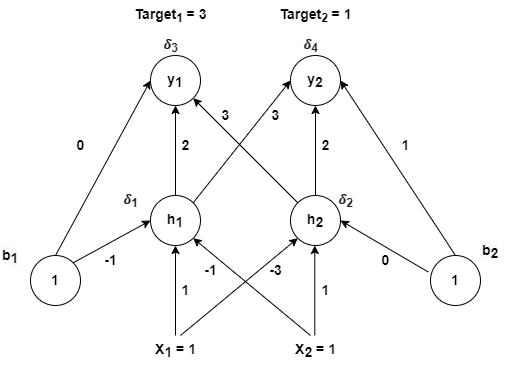
\includegraphics[scale=0.6]{backprop.png}

		      \label{fig:backprop}
	      \end{figure}

	      \begin{tcolorbox}[title={Solution}]
		      Following the learning rule
		      $$ w_{ij} := w_{ij}- \alpha \frac{\partial J}{\partial w_{ij}} =
			      w_{ij} + \alpha_j z_i $$
		      and the definitions of $\delta_j$
		      $$
			      \begin{aligned}
				      \delta_j & = (t_j - y_j)                    & (\text{output unit}) \\
				      \delta_j & = g'(a_j) \sum_k \delta_k w_{jk} & (\text{hidden unit})
			      \end{aligned}
		      $$
		      We have the following values

		      \textbf{Neurons:}

		      $h_1 = 0$

		      $h_2 = 0$

		      $y_1 = 0$

		      $y_2 = 1$

		      \textbf{Deltas:}

		      $\delta_1 = 0$

		      $\delta_2 = 0$

		      $\delta_3 = 3$

		      $\delta_4 = 0$

		      \textbf{Weights:}

		      % layer 1
		      $x_1$ to $h_1 = 1$

		      $x_1$ to $h_2 = -3$

		      $x_2$ to $h_1 = -1$

		      $x_2$ to $h_2 = 1$

		      $b_1$ to $h_1 = -1$

		      $b_2$ to $h_2 = 1$

		      % layer 2
		      $b_1$ to $y_1 = 0 \rightarrow 3$

		      $b_2$ to $y_2 = 1$

		      $h_1$ to $y_1 = 2$

		      $h_1$ to $y_2 = 3$

		      $h_2$ to $y_1 = 3$

		      $h_2$ to $y_2 = 2$

	      \end{tcolorbox}

\end{enumerate}
